Per lo sviluppo del gioco si è scelto di utilizzare il pattern MVC in quanto si vuole avere una separazione pulita tra la parte logica e la parte di visualizzazione. In questo modo si lascia aperta la possibilità di avere diversi tipi di interfaccia grafica.

Inoltre si è scelto di utilizzare un event-loop per gestire la ricezione di input utente, l'update della parte logica e l'update della parte di interfaccia grafica. 

Di seguito è riportato un diagramma che illustra le classi principali per la comunicazione tra Model-View-Controller.

\begin{figure}[H]
  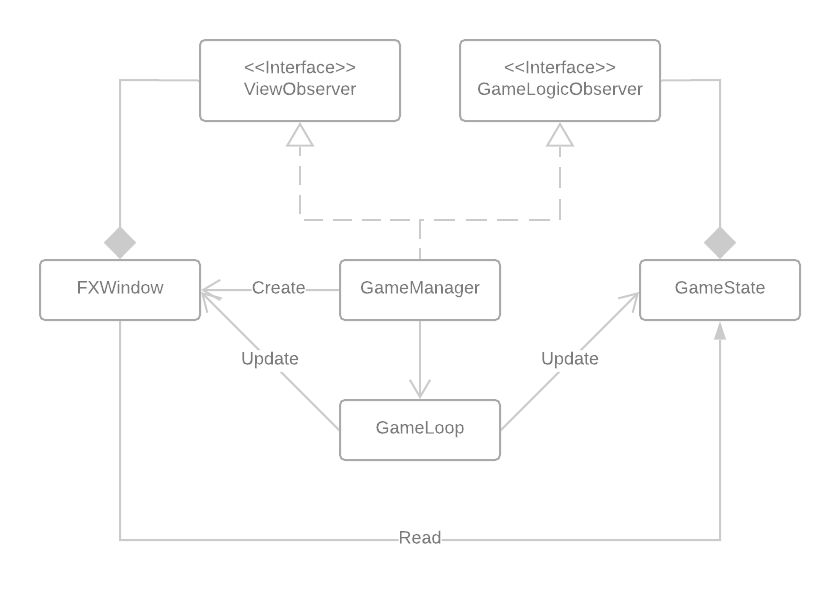
\includegraphics[width=15cm]{res/MVC_Diagram.png}
  \caption{Utilizzo pattern MVC}
\end{figure}